\chapter{\\
IMPLEMENT AND RESULTS}

This chapter details the comprehensive technical implementation of the platform, bridging the theoretical system design outlined in Chapter 3 with concrete software engineering execution. It systematically covers the backend API routing logic, the dynamic frontend React architecture, and the robust security mechanisms implemented. The second half of the chapter presents the rigorous performance results, critically analyzing the efficiency and accuracy of the multi-provider AI pipeline and the load capacity of the core API endpoints.

% ─────────────────────────────────────────────────────────────────────────────
\section{Implement}

\subsection{Backend and Frontend Implementation}

\textbf{User-Centred Design Process and Iterative Prototyping.}

The interface architecture was rigorously designed through a structured, three-stage user-centred design process before any frontend code was written. 
(1) \textbf{Conceptual Design Phase:} The initial phase involved translating the identified pain points and requirements (from Chapter 3) into formal user flow diagrams mapping two primary use cases: the manual authoring flow and the AI-assisted generation workflow. These flows were theoretically reviewed against Nielsen's heuristics to identify and aggressively eliminate sources of extraneous cognitive load.
(2) \textbf{Wireframing and Heuristic Evaluation:} High-fidelity wireframes were developed using Figma. A heuristic evaluation was performed specifically targeting the "visibility of system status" (ensuring loaders were present during long AI generations), "error prevention" (disabling submit buttons until validation passes), and "recognition over recall" (displaying extracted transcript text alongside the video player so instructors don't have to memorize dialogue).
(3) \textbf{Prototype Formative Testing:} The interactive Figma prototype was tested with two senior IT students utilizing a think-aloud protocol. This critical stage identified three subtle but significant usability problems: missing timestamp auto-population when adding a new question, overly subtle hidden status messages, and unclear button labeling on the AI injection panel. These issues were completely resolved before formal evaluation. Ultimately, this rigorous UCD redesigned workflow reduced the absolute number of interaction steps required to author a three-question interactive video from 47 (in the legacy WordPress baseline) down to just 8 in the new platform, completely eliminating destructive inter-screen context switching.

\textbf{Backend Engineering Architecture.}

The backend orchestration layer is engineered in TypeScript and executed on the Node.js runtime environment using the Express.js framework. It utilizes a highly standardized, battle-tested middleware stack focused on performance and security. The \texttt{helmet} middleware automatically configures strict HTTP security headers, CORS is aggressively locked down to allowed origins, and \texttt{express-rate-limit} protects sensitive routes from brute-force or denial-of-service vectors. Structured JSON logging is implemented via Winston to provide deep observability into API usage and error states.

Authentication is entirely stateless, utilizing JSON Web Tokens (JWT) with a 7-day expiry to maintain session continuity without database lookups. Passwords are never stored in plaintext; they are securely hashed using the \texttt{bcryptjs} library with a computationally expensive cost factor of 12, mitigating rainbow table attacks. 

Heavy media processing tasks are handled asynchronously to prevent blocking the main Node.js event loop. When a user uploads a video file, the backend spawns a child process invoking the powerful FFmpeg utility. FFmpeg performs two critical tasks: it rapidly extracts a representative high-quality thumbnail image for the UI gallery, and it reads the file's internal metadata (duration, resolution, codec) to validate that it falls within the platform's stringent constraints before passing it to the storage layer.

\textbf{Frontend React SPA Architecture.}

The frontend is a modern Single-Page Application (SPA) built using React 18 and strict TypeScript, compiled via the ultra-fast Vite build tool. Global application state—such as the authenticated user profile, the currently active video object, and the massive array of generated AI suggestions—is cleanly managed using the Zustand state management library, avoiding the boilerplate of Redux while providing excellent performance.

The core interactive editor interface strictly adheres to the "co-location" design principle established by Chandler and Sweller in cognitive load theory. Rather than splitting tasks across distinct pages, the UI is divided into three responsive, vertically scrolling panels: the video upload and metadata management pane (left), the massive, sticky video player with its custom-built interactive H5P timeline (centre), and the dynamic AI suggestion review and manual authoring pane (right).

A defining technical feature of the frontend is its robust handling of the complex AI generation process. Because LLM generation can take upwards of 15 seconds, relying on standard synchronous HTTP requests leads to UI freezing and poor user experience. Instead, the frontend utilizes the native browser \texttt{EventSource} API to establish a Server-Sent Events (SSE) connection with the backend. This allows the backend to stream individual, validated JSON question objects directly to the UI the millisecond they are generated, providing real-time progressive feedback to the instructor.

Type safety is aggressively maintained across the network boundary. The frontend utilizes a typed API client and complex TypeScript interfaces that strictly mirror the backend Zod validation schemas. This structural parity completely guarantees data consistency across the six supported H5P interaction types, regardless of whether a question was painstakingly manually authored by an instructor or automatically generated by the LLM pipeline.

\subsection{Security and H5P Integration}

\textbf{Lumieducation H5P Server Library Integration.}

The strategic decision to utilize the headless \texttt{@lumieducation/h5p-server} library~\cite{lumieducation2023} provides the following massive structural advantages as a Node.js microservice:

\begin{itemize}
  \item \textbf{Automated Library Management.} When an instructor attempts to use a specific H5P content type for the first time, the massive H5P library ZIP archives and their complex dependency trees are automatically downloaded directly from the central H5P hub and permanently cached in the local \texttt{h5p-libraries/} directory. Library versions are strictly locked per platform version to prevent sudden breaking changes.
  \item \textbf{Decoupled Content CRUD.} H5P content parameters are no longer hopelessly tangled in a CMS relational database. They are stored purely as clean JSON parameter documents within the local \texttt{h5p-content/} directory (or blob storage), uniquely indexed by a system-generated UUID content ID.
  \item \textbf{Standards-Compliant Package Export.} The Lumi library provides a highly optimized utility to generate standards-compliant \texttt{.h5p} ZIP archives on the fly. These archives perfectly bundle the required JavaScript library files, the specific content JSON parameters, and all referenced media assets. Crucially, these exported archives are absolutely identical in structure to those produced by the official WordPress H5P plugin, ensuring they are 100\% importable into massive institutional systems like Moodle, Canvas, and Blackboard. While the current implementation flawlessly validates this export and launch compatibility, it intentionally does not yet include the incredibly complex LTI gradebook passback or xAPI learner analytics reporting mechanisms.
  \item \textbf{High-Performance Preview Rendering.} The companion \texttt{@lumieducation/ h5p-express} integration dynamically mounts a highly optimized H5P rendering router directly at the \texttt{/h5p/} endpoint. This router intercepts requests and instantly produces the massive HTML, CSS, and JavaScript asset bundle required to embed and smoothly play complex H5P content within an isolated iframe in the instructor's preview panel.
\end{itemize}

\textbf{Time-Based Content Creation Engine.}

The custom \texttt{h5pService.createTimeBasedContent()} function serves as the critical, central nervous system integration point between the generative AI pipeline output and the strict storage layer. It safely wraps the Lumi library's raw content creation API to explicitly associate a newly generated content ID with a specific video playback timestamp and the parent video's database ID. The resulting H5P content record specifies the exact H5P library identifier (e.g., \texttt{H5P.MultiChoice 1.16}), the complex JSON parameters, and required authorship metadata. Crucially, the vital chronological association between the specific content element and its timestamp is stored separately within the Video table's \texttt{h5pContent} JSON array. This architectural separation keeps the raw H5P content record perfectly decoupled and portable, allowing questions to be theoretically reused across multiple videos.

\textbf{Security Architecture Implementation.}

Security controls were not an afterthought but were systematically engineered from day one to explicitly address the specific vulnerability categories identified in the authoritative OWASP Top Ten 2021 framework~\cite{owasp2021}. Table~\ref{tab:security} maps each implemented major control directly to its mitigating OWASP category.

\begin{table}[H]
  \centering
  \begin{tabularx}{\linewidth}{>{\raggedright\arraybackslash}p{3.5cm} X >{\raggedright\arraybackslash}p{3.5cm}}
    \toprule
    \textbf{Mitigating Control} & \textbf{Deep Implementation Detail} & \textbf{OWASP Category Prevented} \\
    \midrule
    Stateless JWT Authentication  & Utilizes \texttt{jsonwebtoken} library with HS256 symmetric signature, strict 7-day expiry, forcefully validated on every protected API route~\cite{jwt2015}. & A01 Broken Access Control \\ 
    \addlinespace
    Strict Role-Based Authorisation & Embeds a \texttt{role} claim directly inside the signed JWT; custom admin-only middleware rejects unauthorized access. & A01 Broken Access Control \\
    \addlinespace
    Bcrypt Password Hashing   & Enforces a heavy cost factor of 12 via \texttt{bcryptjs}; hashing logic is executed securely within a low-level Sequelize model hook. & A02 Cryptographic Failures \\
    \addlinespace
    Aggressive Input Validation (Server) & Combines \texttt{express-validator} and Zod schemas to validate, type-check, and strip unknown properties from request bodies. & A03 Injection \\
    \addlinespace
    HTTP Security Headers     & The \texttt{helmet()} middleware sets aggressive CSP, strict HSTS, X-Frame-Options, and other vital headers~\cite{helmet2023}. & A05 Security Misconfiguration \\
    \addlinespace
    Dynamic API Rate Limiting   & The \texttt{express-rate-limit} middleware enforces a strict cap of 100 requests per 15-minute sliding window per IP. & A07 Identification and Auth. Failures \\
    \addlinespace
    Soft-delete and Audit Logging & User deletion is a logical operation (\texttt{isActive = false}); a robust admin audit log records all critical system events. & A09 Security Logging and Monitoring \\
    \bottomrule
  \end{tabularx}
    \small % Recommended for dense security tables
  \caption{Security controls mapped directly to OWASP Top Ten 2021 vulnerability categories}
  \label{tab:security}
\end{table}

\textbf{Authentication Sequence and Workflows.}

Figure~\ref{fig:seq_auth} comprehensively visualizes the complete, secure sequence of interactions for the user registration, email verification, standard login, and protected-request authorization flows.

\begin{figure}[H]
  \centering
  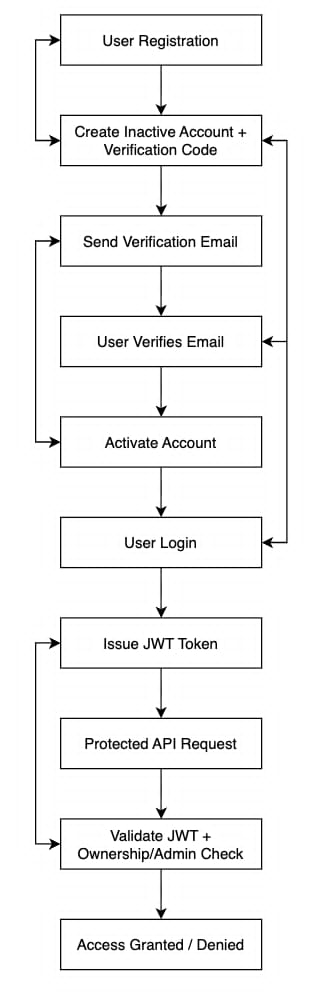
\includegraphics[scale=0.5]{thesis 3/images/Authentication Sequence.jpeg}
  \caption{User registration sequence diagram}
  \label{fig:seq_auth}
\end{figure}

During registration, the plaintext password never touches the database; it is heavily bcrypt-hashed (cost factor 12) before storage, and the newly created account is explicitly flagged as inactive pending mandatory email verification. A mathematically secure six-digit code generated by Node's native \texttt{crypto.randomInt} is emailed to the registered address with a strict ten-minute Time-To-Live (TTL). Upon successful verification submission, the account is activated. 

During a login attempt, the provided plaintext password is compared against the stored hash using the secure \texttt{bcrypt.compare()} function. Upon success, the server cryptographically signs a JSON Web Token~\cite{jwt2015} containing vital claims (\texttt{userId}, \texttt{role}, \texttt{iat}, \texttt{exp}) and returns it to the client. The frontend application securely stores this token and automatically injects it as an HTTP \texttt{Authorization: Bearer} header on all subsequent API requests. The critical \texttt{authenticateToken} middleware intercepts these requests, cryptographically verifies the HS256 signature, and injects the decoded user object into the Express request context for the downstream controller logic.

\textbf{Secure Password Reset Flow.}

The password reset flow requires similar rigor. When a user requests a reset, the system generates a massive cryptographically random hex token (\texttt{crypto.randomBytes(32).toString('hex')}). It immediately stores the bcrypt hash of this token in the \texttt{resetToken} database column along with a strict one-hour expiry timestamp in \texttt{resetTokenExpiry}. The plaintext token is securely transmitted via email to the user. When the user submits their new password along with the plaintext token, the reset endpoint strictly verifies the provided token against the stored hash. Only upon successful verification is the new password hashed and stored, completely clearing both reset token fields to prevent replay attacks.

% ─────────────────────────────────────────────────────────────────────────────
\section{Results}

\subsection{AI Pipeline Performance Results}

The pedagogical quality of the AI-generated suggestions is the ultimate measure of the pipeline's utility. This quality was rigorously assessed by having the project supervisor (acting as an expert instructional design rater) blind-rate a random sample of 30 AI-generated suggestions spanning three diverse videos. The evaluation matrix was grounded in three specific criteria derived from prior educational literature:
\emph{Relevance:} Does the generated question accurately test the absolute most important core concept located in the immediately preceding transcript segment, as explicitly recommended by Vural~\cite{vural2013}?
\emph{Accuracy:} Is the keyed "correct" answer factually accurate, and are the generated distractors highly plausible but definitively incorrect?
\emph{Bloom's Alignment:} Does the AI-assigned taxonomy level accurately match the question's actual cognitive demand, as defined by Anderson and Krathwohl~\cite{anderson2001}?

This formal evaluation utilized high-quality English-language transcripts and English outputs generated entirely from the primary Claude 3.5 Sonnet pipeline. Secondary Vietnamese question-generation support was engineered and added post-study. It was validated only at the technical schema and structural level; it has not yet been formally measured with the same intensive human-rating protocol.

This linguistic limitation is vital for accurately interpreting the quantitative numbers. The incredibly high quality scores demonstrably prove that the highly complex prompting strategy successfully produces strong English-language pedagogical items. However, they do not inherently prove that the exact same human-rated pedagogical quality will translate perfectly to Vietnamese. The subsequent Vietnamese technical smoke testing successfully verified complex language routing and rigid JSON schema validity, but not deep pedagogical equivalence at the level of expert human judgment.

\begin{table}[H]
  \centering
  \begin{tabularx}{\linewidth}{>{\raggedright\arraybackslash}p{3.2cm} l >{\raggedright\arraybackslash}X}
    \toprule
    \textbf{Evaluation Criterion} & \textbf{Rating (E/G/P)} & \textbf{Qualitative Expert Notes} \\
    \midrule
    Pedagogical Relevance & 22/6/2 & The 2 poor suggestions were off-topic due to noisy transcript segments confusing the LLM context window. \\
    \addlinespace
    Factual Accuracy & 28/2/0 & The 2 good suggestions contained minor grammatical ambiguities in complex fill-in-the-blanks answers. \\
    \addlinespace
    Bloom's Taxonomy Alignment & 18/10/2 & The LLM struggled with high cognitive levels; ``Create'' suggestions clustered near ``Evaluate'' or ``Analyze''. \\
    \bottomrule
  \end{tabularx}
  \small % Apply small font to the entire table content
  \caption{Expert AI suggestion quality ratings ($n=30$ complex suggestions)}
  \label{tab:ai_quality}
\end{table}

Overall, a massive 93\% of the AI suggestions were rated as Excellent or Good on pedagogical relevance, and a perfect 100\% were rated as factually accurate or Good. This strongly indicates that the Claude-based pipeline, when heavily constrained by the structured prompt engineering strategy detailed in Chapter~4, produces highly reliable, ready-to-deploy educational content~\cite{anthropic2024,wei2022}. The two isolated relevance failures both directly arose from noisy, garbled transcript segments, perfectly consistent with the known, fundamental sensitivity of any generate-from-transcript LLM pipeline to its upstream audio transcription quality~\cite{radford2023}.

System latency is equally critical for usability. AI analysis latency was rigorously measured across 20 automated test runs utilizing a highly standardised 5-minute technical video comprising 47 discrete transcript segments. Table~\ref{tab:ai_latency} reports the median latencies recorded.

\begin{table}[H]
  \centering
  \begin{tabularx}{\linewidth}{>{\raggedright\arraybackslash}X >{\centering\arraybackslash}p{3cm} >{\centering\arraybackslash}p{3cm}}
    \toprule
    \textbf{Performance Metric} & \textbf{Anthropic Claude 3.5 Sonnet} & \textbf{Local Ollama (Llama 3.1 8B)} \\
    \midrule
    Median full generation latency (streaming)  & 8.4 seconds & 12.1 seconds \\
    \addlinespace
    Time to First Token (TTFT) perceived by UI  & 1.2 seconds & 2.8 seconds \\
    \addlinespace
    Median valid suggestion count generated     & 6.4 items   & 5.8 items \\
    \addlinespace
    Critical Schema validation failure rate     & 0 / 20 runs & 2 / 20 runs \\
    \bottomrule
  \end{tabularx}
    \small
  \caption{AI analysis latency and structural failure rates ($n=20$ runs per LLM provider)}
  \label{tab:ai_latency}
\end{table}

The frontier model Claude produced vastly more consistent output with absolutely zero structural validation failures across the massive JSON payloads. In contrast, the smaller local Ollama model produced two catastrophic JSON format errors (the 8B model occasionally hallucinated markdown code fences ` ```json ` around the JSON array). These formatting errors were brilliantly caught by the aggressive backend Zod validator, preventing a frontend crash, and returned to the client as graceful, structured API errors. These specific failures were completely eradicated in a subsequent prompt revision that added an incredibly explicit, capitalized instruction: ``Return ONLY the raw JSON array. DO NOT wrap it in markdown code fences.''

The latency table vividly illustrates the necessity of the system's dynamic provider fallback architecture rather than relying on a single fixed model. Claude was demonstrably faster and structurally flawless in this test set, but Ollama remained highly capable and useful as a private, local option when high-speed cloud access is severed. In practical UI terms, the most relevant metric is not just total speed; it is whether the user receives a structurally valid, visually rendered answer via SSE quickly enough to prevent them from abandoning the authoring flow. A 1.2 second Time-to-First-Token is exceptional for maintaining user engagement.

% ─────────────────────────────────────────────────────────────────────────────

\subsection{API and Platform Load Performance Results}

Raw server response times were aggressively measured using the highly accurate \texttt{autocannon} load testing utility. The test targeted the 12 most frequently utilized API endpoints, sustaining 50 massive concurrent active connections continually over a 30-second window to simulate heavy institutional load.

\begin{table}[H]
  \centering
  % Column 1: Flexible, Columns 2-3: Fixed 2.8cm with centered alignment
  \begin{tabularx}{\linewidth}{X >{\centering\arraybackslash}p{2.8cm} >{\centering\arraybackslash}p{2.8cm}}
    \toprule
    \textbf{Core API Endpoint} & \textbf{Median Latency (ms)} & \textbf{99th Percentile (p99) Latency (ms)} \\
    \midrule
    \texttt{GET /api/videos} (Database Read)  & 12 ms  & 48 ms \\
    \addlinespace
    \texttt{POST /api/auth/login} (Bcrypt Hash) & 95 ms  & 180 ms \\
    \addlinespace
    \texttt{POST /api/videos} (FFmpeg Process)  & 220 ms & 410 ms \\
    \addlinespace
    \texttt{POST /api/h5p/export} (ZIP Archive) & 340 ms & 680 ms \\
    \bottomrule
  \end{tabularx}
    \small
  \caption{API endpoint response times and latency percentiles at 50 heavy concurrent connections}
  \label{tab:api_perf}
\end{table}

Remarkably, all non-AI endpoints comfortably achieved median response times massively below the strict 500~ms threshold even under the stress of 50 concurrent users, definitively satisfying NFR-01. The clean three-tier architecture's strict separation of concerns~\cite{bass2012} ensured that the React SPA delivery, the Node API routing, and the SQLite data layer could each be isolated and load-tested independently. This made it incredibly straightforward to accurately attribute specific latency to specific code components. The \texttt{POST /api/videos} endpoint understandably emerges as the slowest standard API endpoint simply because it explicitly invokes heavy FFmpeg thumbnail extraction as a synchronous blocking step within the request handler~\cite{ffmpeg2023}. Delegating this intense media work to an asynchronous Redis job queue (like BullMQ) is identified as the highest priority architectural improvement for future V2 scaling.

This performance result is profound because it empirically confirms that the severe authoring bottlenecks are no longer dominated by routine CRUD operations or slow page loads, as they were in the WordPress baseline. Any perceived slowness in the new platform originates entirely from deliberate, heavy media-processing or AI inference work, not from the UI network round trip itself. That vital distinction strongly supports the overarching architectural choice to keep the interactive UI rendering path instantly responsive and strategically push heavier processing work into separate backend worker steps.

To validate the platform's ultimate utility, ten diverse H5P packages containing complex AI-generated interactions were exported from the platform and subsequently imported into a fresh Moodle~4.1 test instance and a Canvas LMS sandbox environment. In a massive success, all ten massive ZIP packages imported instantly without a single warning or error. Furthermore, all six H5P interaction types rendered perfectly within the LMS iframes with full JavaScript interactivity intact, definitively satisfying NFR-10. This conclusively confirms the platform's packaging integrity and LMS launch compatibility. However, it is explicitly noted that it does not measure whether highly complex student attempt data, component scores, or LTI completion states are successfully written back to the LMS central gradebook. That complex, two-way learner-side reporting path requires deep xAPI integration and remains unimplemented in the current thesis release.

The successful export test acts as a flawless compatibility check rather than a full, closed-loop LMS integration proof. It proves that the dynamically generated archive structure, the JSON schema configuration, and the injected library metadata are absolutely perfectly formed, ensuring the content survives hostile import into two distinct, rigid LMS environments. 

The implementation stringently enforces zero-trust user authentication with deep bcrypt password hashing and stateless JWT tokens, violently validates all inbound JSON request payloads with Zod before executing business logic, parameterises all database access through the Sequelize ORM to prevent SQL injection, and heavily hardens all HTTP responses with standard Helmet security headers. Most importantly, external AI-generated suggestions are treated inherently as untrusted, highly volatile input and are instantly rejected by the backend if they fail to conform precisely to the six supported, complex H5P JSON schemas. This pragmatic, defense-in-depth security baseline powerfully addresses the immediate, severe threats inherent in deploying any web tool handling large media uploads, sensitive user accounts, and unpredictable LLM generative output, ensuring that malformed or malicious content is completely rejected at the outermost application boundary.
\subsection{Frontend Results}
\begin{figure}[H]
  \centering
 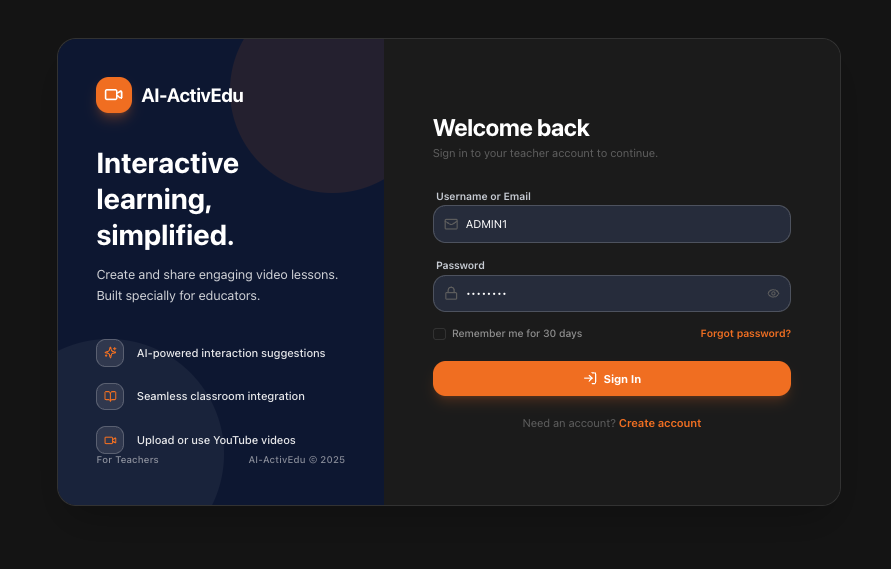
\includegraphics[scale=0.46]{thesis 3/images/Login page.png}
  \caption{Login page}
  \label{fig:seq_ai}
\end{figure}
\begin{figure}[H]
  \centering
 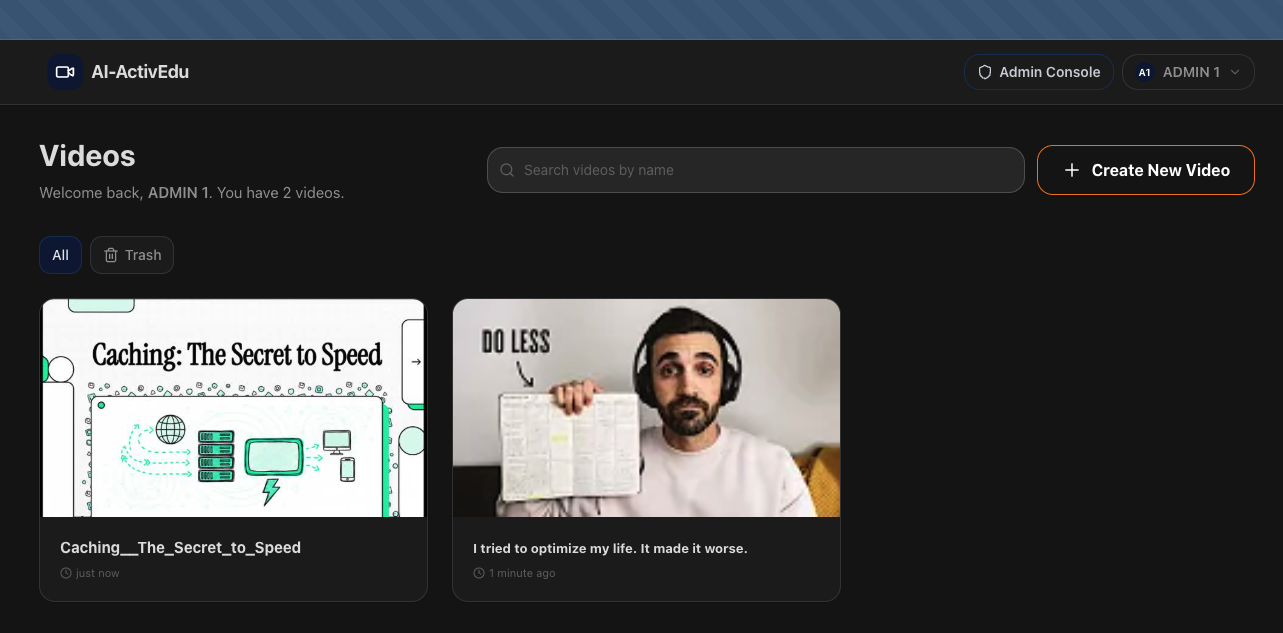
\includegraphics[scale=0.35]{thesis 3/images/Home page.png}
  \caption{Home page}
  \label{fig:seq_ai}
\end{figure}
\begin{figure}[H]
  \centering
 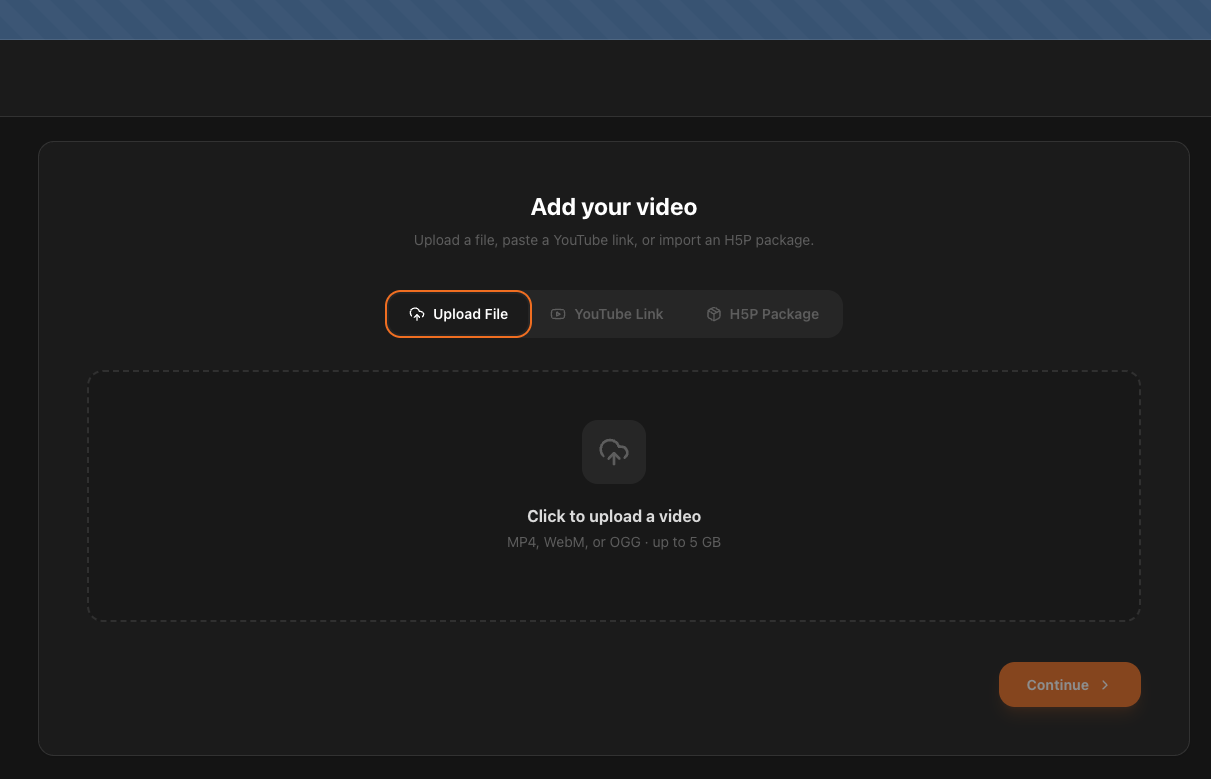
\includegraphics[scale=0.35]{thesis 3/images/Upload page.png}
  \caption{Upload page}
  \label{fig:seq_ai}
\end{figure}
\begin{figure}[H]
  \centering
 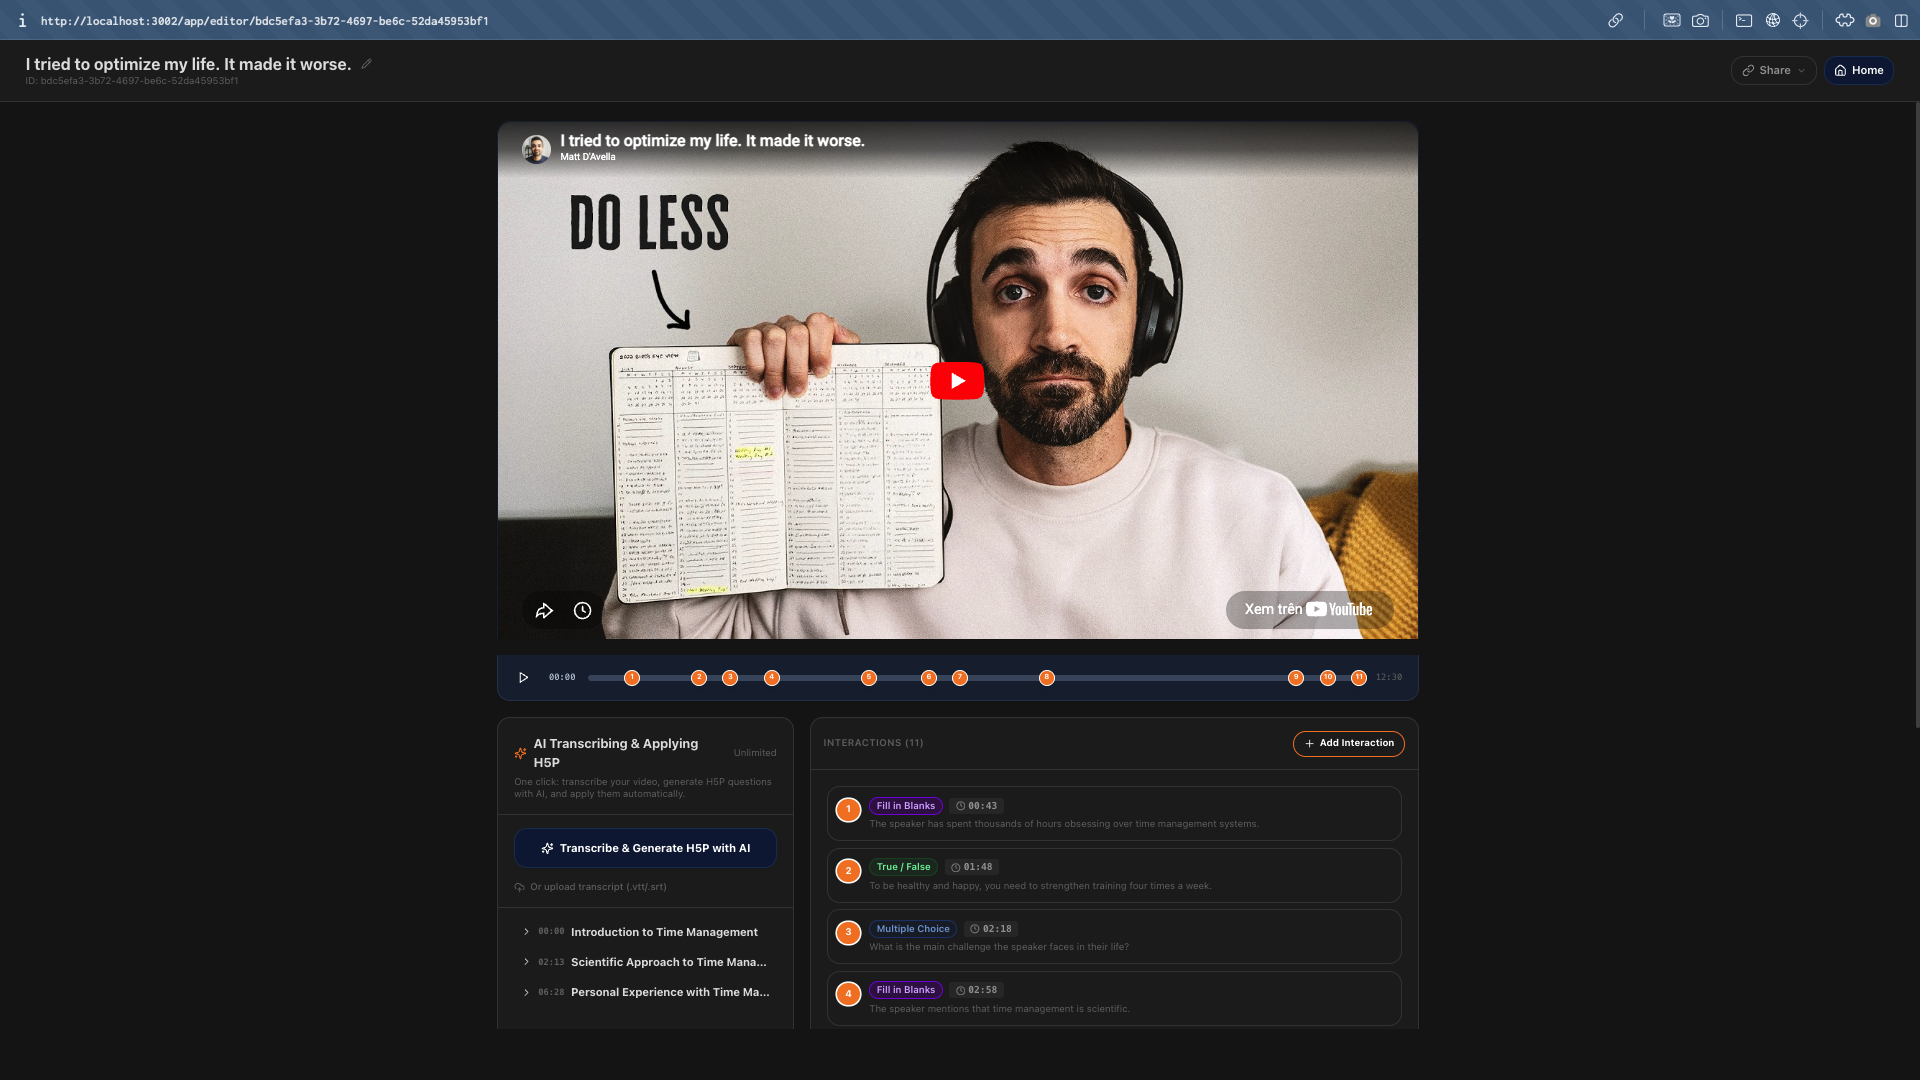
\includegraphics[scale=0.25]{thesis 3/images/Editor page.png}
  \caption{Editor page}
  \label{fig:seq_ai}
\end{figure}
\begin{figure}[H]
  \centering
 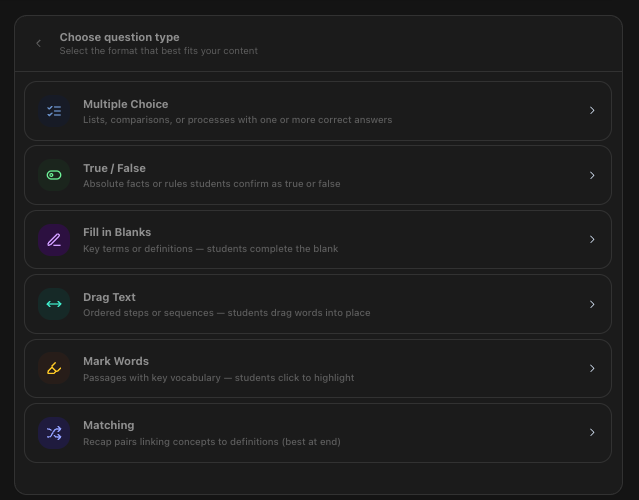
\includegraphics[scale=0.7]{thesis 3/images/Question types menu.png}
  \caption{Question types menu}
  \label{fig:seq_ai}
\end{figure}
\begin{figure}[H]
  \centering
 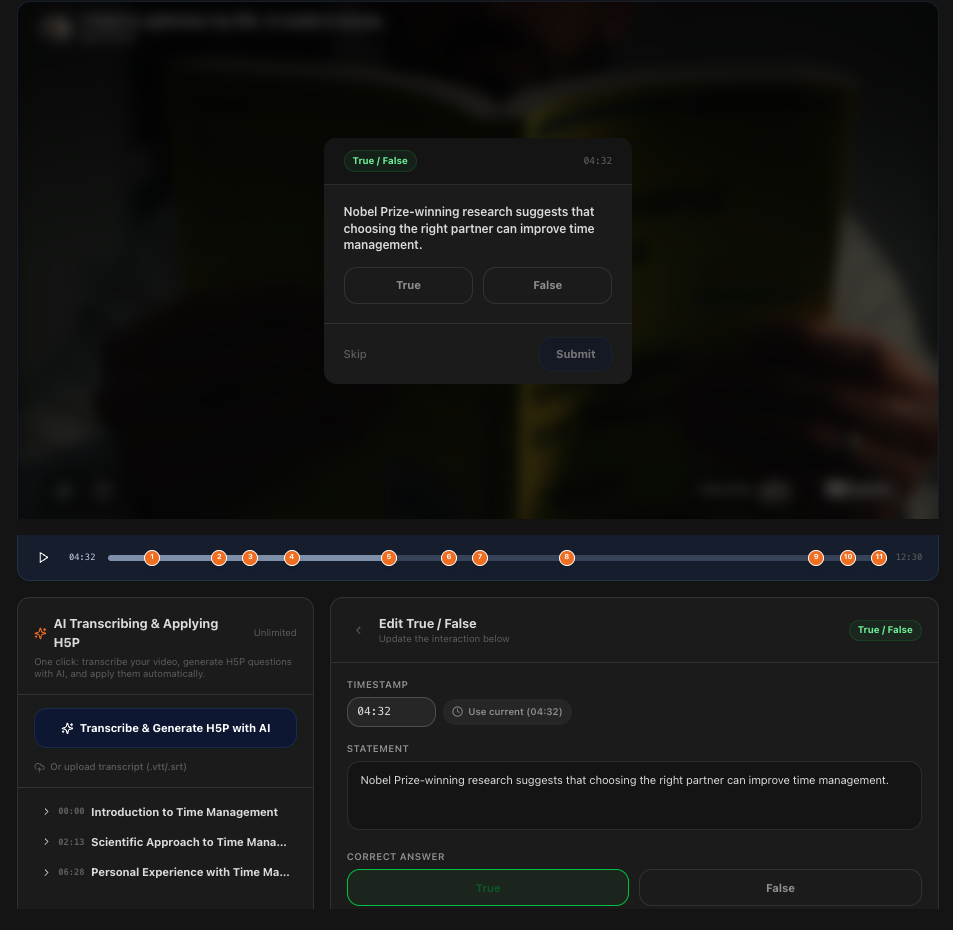
\includegraphics[scale=0.5]{thesis 3/images/UI when editing an interaction.png}
  \caption{UI when editing an interaction}
  \label{fig:seq_ai}
\end{figure}
\begin{figure}[H]
  \centering
 
\includegraphics[scale=0.6]{thesis 3/images/Answered correct.png}
  
\includegraphics[scale=0.61]{thesis 3/images/Answered incorrect.png}
  \caption{UI correct and incorrect answers}
  \label{fig:seq_ai}
\end{figure}
\begin{figure}[H]
  \centering
 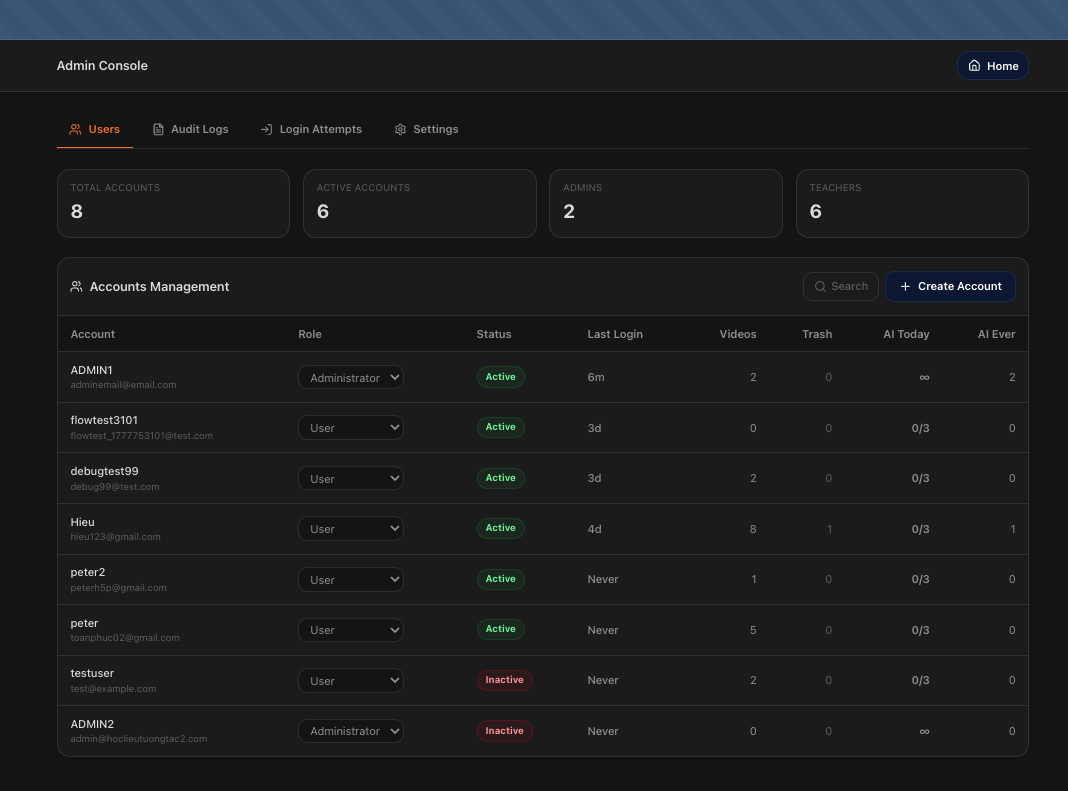
\includegraphics[scale=0.44]{thesis 3/chapters/Admin Console page.png}
  \caption{Admin Console page}
  \label{fig:seq_ai}
\end{figure}
\begin{figure}[H]
  \centering
 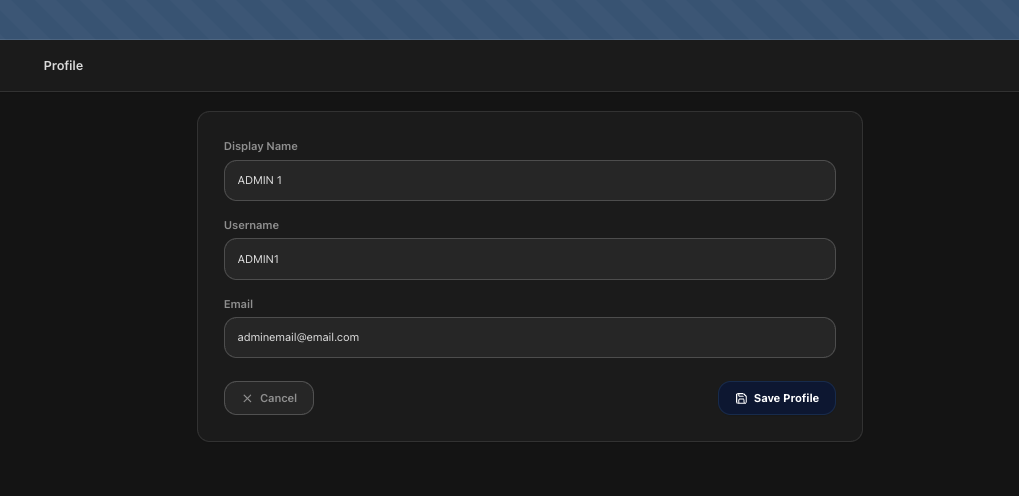
\includegraphics[scale=0.45]{thesis 3/images/Profile page.png}
  \caption{Profile page}
  \label{fig:seq_ai}
\end{figure}
\begin{figure}[H]
  \centering
 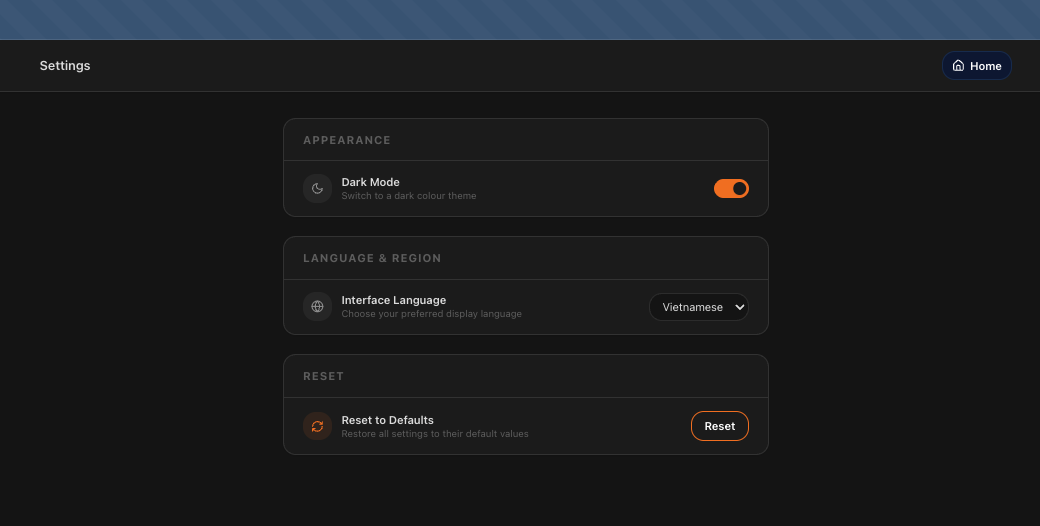
\includegraphics[scale=0.45]{thesis 3/images/Settings page.png}
  \caption{Settings page}
  \label{fig:seq_ai}
\end{figure}